\section{Theory}
\label{sec:theory}

% The first derivative primarily tells us about the direction the function is going. That is, it tells us if the function is increasing or decreasing.

% the second derivative tells us if there is an increase in the increase of the function
This section will investigate the theory aspects of solving the Art Gallery Problem using gradient descent. Namely, we will explain what the optimisation function in the context of the Art Gallery problem is, and how it can be solved with gradient descent. We will initially apply gradient descent to only one guard, then extend it to multiple guards.

\subsection{Guarding the Polygon with One Point}

First, we will explore how gradient descent can be applied for the case that we want to guard the polygon using only one guard.

\subsubsection{Gradient Descent}

Let $P$ be a polygon and $g = (x, y) \in P$ a guard. We are interested in computing the best direction for moving $g$ inside $P$ such that the visibility area $\mathit{Vis}(g)$ increases. That is, exploring what would be a better position $g'$ to move $g$ to such that $g$ ``sees more'' of the polygon $P$. 

We define $f(g) = \text{Area}(g)$ as the area seen by a guard $g$. Let $\bigtriangledown \text{Area}_r(g)$ be the local change in the area guarded by point $g$ around a reflex vertex $r$ seen by guard $g$, thus $r \in \mathit{Vis(g)}$. Given all reflex vertices $i$, the total (global) change in the area seen by $g$ can be thus summed up to $\text{Area}(g) = \sum_i \text{Area}_i(g)$. Figure \ref{fig:sumf} offers an example for this case for a polygon $P$ and its reflex vertices $r_1$ and $r_2$. The polygon $P$ is guarded by $g$, and its position is modified to $g'$ by a small change $\partial y$ in its $y$-coordinate. The visibility areas of $g$ are $Area_{r_1}$ and $Area_{r_2}$ around reflex vertices $r_1$ and $r_2$, respectively. In this way, the total change in the visibility area of $g$ is computed as $\bigtriangledown \text{Area}(g) = \bigtriangledown \text{Area}_{r_1}(g) + \bigtriangledown \text{Area}_{r_2}(g)$.

Thus, we consider $f(g)$ as the continuous objective function of the Art Gallery Problem. We can then use gradient descent as a method to optimise the objective function $f$. We will define below what the methodology of gradient descent is comprised of.

\begin{figure}[h!]
    \centering
    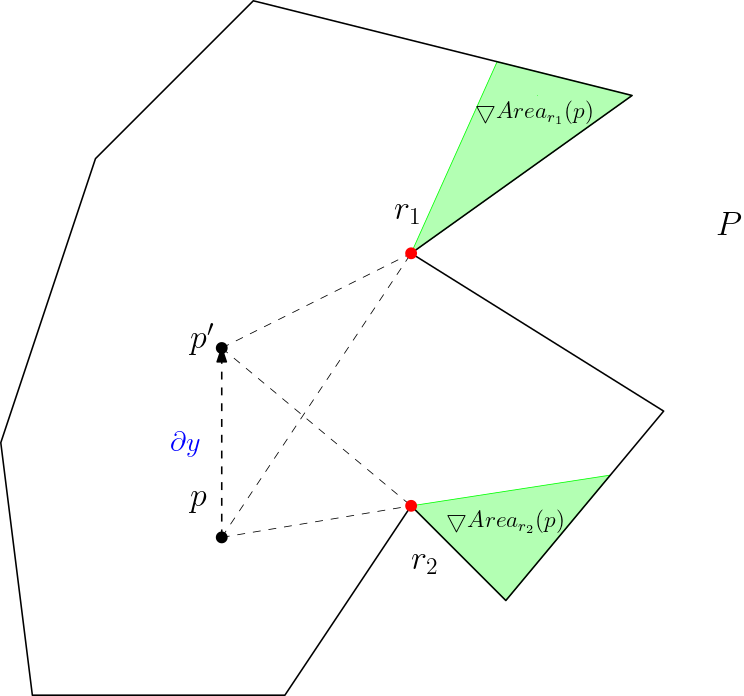
\includegraphics[width=0.4\textwidth]{theory/sumf.png}
    \caption{Global change in the area seen by $g$ when moved by $\partial y$ to a new position $g'$.}
    \label{fig:sumf}
\end{figure}


Let $\bigtriangledown f$ be the gradient of $f$. The gradient then indicates the direction of the steepest descent for the objective function $f(g)$.
The learning rate (step size) $\alpha$ is the size of the steps taken to reach the optimum. It is typically a small value, and it is evaluated and updated based on the behaviour of the optimisation function. 

After the gradient $\bigtriangledown f$ is computed, we can use it to calculate the new optimised position $g'$ of guard $g$: $$g' = g + \alpha\bigtriangledown f.$$


In later sections we will experiment with various learning rates. As such, we will explore how they influence the performance of our algorithm in relation to different test polygons. 

\newpage
\subsubsection{Computing the Gradient}

Given that $f$ is a function that describes the visibility area of a point $g$, we first need to define how its gradient is computed. We will simplify the gradient computation without losing generality. As such, we will rotate the plane with rotation matrix $R$, so that $g$ and any reflex vertex $r$ have the same $x$-coordinate. In this way, we only need to compute the gradient when we vary the $y$-coordinate. The computation of the gradient remains the same regardless of the rotation applied to the plane.


We will use the notation $\frac{\partial f}{\partial y}$ to denote the change in the visibility area $f(g)$ when the plane is rotated and then the $y$-coordinate is modified by a small amount $\partial y \rightarrow 0$. In this way, we define 

\begin{equation}
    \bigtriangledown f = \left(\frac{\partial f}{\partial x}, \frac{\partial f}{\partial y}\right)^\intercal \label{eq:gradient}
\end{equation}

to be the gradient of $f$ given that $P$ is guarded by a point $g$. 

We will now create a canonical geometrical construction that allows us to further define and compute $\bigtriangledown f$. In this case, we consider the normalised length of the gradient as $||~\bigtriangledown~f||~=~1$. This canonical construction is displayed in Figure \ref{fig:gradient}. 
% We will then generalise this case to multiple reflex vertices and guards.

\begin{figure}[h!]
    \centering
    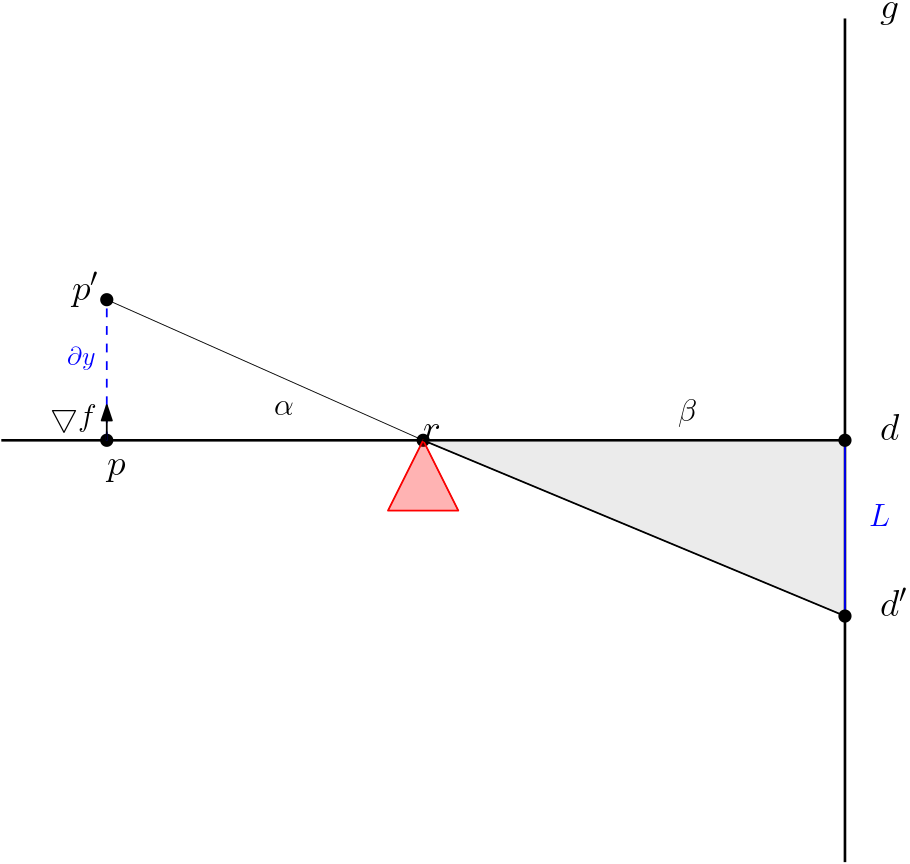
\includegraphics[width = 0.6\textwidth]{theory/gradient2.png}
    \caption{Canonical gradient construction for when the position of $g$ is varied by a small amount $\partial y$ around reflex vertex $r$ to the new position $g'$.}
    \label{fig:gradient}
\end{figure}

Take a boundary line segment of $P$, $r$ a reflex vertex inside $P$ and $g$ a guard whose optimal position we are interested in. The reflex vertex $r$ is seen by $g$. Let $\overline{pr} = a$ be known, and let $\triangle rpp' = \triangle_2$. Similarly, let $b$ be the known distance between $r$ and the polygon boundary in question.


Let $\partial y$ be an extremely small change in the $y$-coordinate of $g$. Let $g'$ be the new position of $g$ given the change $\partial y$. The point $g'$ can see then up to a new point around $r$ on the polygon boundary. Let thus the new observed segment on the polygon boundary be $L$. As such, let $\triangle_1$ denote the increase in the visibility area of $g$ when it moves to position $g'$:

\begin{equation}
    \bigtriangledown \text{Area}_r = \triangle_1. \label{eq:derivative}
\end{equation}

We are now interested in computing how the area seen by guard $g$ increases given the change $\partial y$ in the position of $g$. The distances $a$ and $b$ are known. As such, we aim at expressing the gradient $\bigtriangledown \text{Area}_r$ for point $g$ and reflex vertex $r \in \mathit{Vis}(g)$ using $a$ and $b$. Since $\bigtriangledown \text{Area}_r$ depends on the change in the coordinates of $g$, computing it is tightly connected to the change in the area of triangle $\triangle_1$. We will proceed to calculate the area of $\triangle_1$ below.

Given that triangles $\triangle_1$ and $\triangle_2$ are square triangles, their areas can be calculated as:

\begin{align*}
    \text{Area}_{\triangle_1} &= \frac{b L}{2},\\ 
    \text{Area}_{\triangle_2} &= \frac{a \partial y}{2}.
\end{align*}


Given that $\overline{gg'}$ is parallel to polygon's boundary, we can use Thales's Theorem in triangles $\triangle_1$ and $\triangle_2$ to compute the length $L$: 

\begin{align}
    % \frac{||\overline{pp'}||}{||\overline{dd'}||} &= \frac a b \\
    \frac{\partial y}{L} &= \frac a b \\
    L &= \frac{b \partial y}{a}. \label{eq:L}
\end{align}

So, the area of $\triangle_1$ can be computed:
\begin{align}
    \text{Area}_{\triangle_1} &= \frac{Lb}{2} \\
    &\overset{(\ref{eq:L})}{=} \frac{\frac{b \partial y}{a}b}{2} \\
    \text{Area}_{\triangle_1} &= \frac{b^2 \partial y}{2a}. \label{eq:ardd}
\end{align}

We can now compute the gradient $\bigtriangledown \text{Area}_r$ in a plane rotated by $R$ for a point $g$ and a reflex guard $r$ seen by $g$ as

\begin{align*}
    R\bigtriangledown \text{Area}_r \overset{(\ref{eq:gradient})}{=} &\left(\frac{\partial f}{\partial x}, \frac{\partial f}{\partial y}\right)^\intercal \\
    \overset{(\ref{eq:derivative})}{=} &\left(0, \frac{\text{Area}_{\triangle_1}}{\partial y}\right)^\intercal \\
    R\bigtriangledown \text{Area}_r \overset{(\ref{eq:ardd})}{=} &\left(0, \frac{b^2}{2a}\right)^\intercal.
    % \bigtriangledown \text{Area}_r = &\left(0, \frac{b^2}{2a}\right)^\intercal.
\end{align*}

% Analogously, if we rotate the plane such that $p$ and reflex vertex $r$ have the same $y$-coordinate, the gradient becomes $$\bigtriangledown f = (\frac{b^2}{2a}, 0)^\intercal.$$

Therefore, for all the reflex vertices $r$ guard $g$ can see, the total gradient $\bigtriangledown f$ becomes the sum of all the partial gradients $\bigtriangledown f_r$ as $$\bigtriangledown f = \sum_{i \in R(g)} \bigtriangledown \text{Area}_i, R(g) = \{\text{reflex vertices of } P \text{ seen by }g\}.$$

\subsubsection{Computing the New Guard's Position}
We can now use the coordinates of the gradient $\bigtriangledown f$ to compute the movement direction of the guard $g$ given all the reflex vertices from $P$ seen by $g$. In order to do so, we will use the construction depicted in Figure \ref{fig:vperp}. 

\begin{figure}[h!]
    \centering
    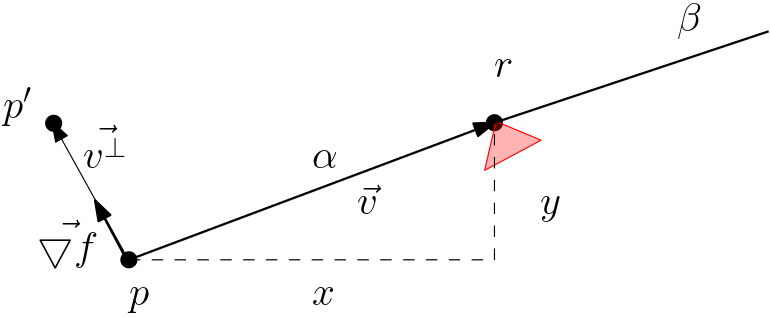
\includegraphics[width = 0.5\textwidth]{theory/v_perp.png}
    \caption{Computing the new position $g'$ of guard $g$ around reflex vertex $r$ based on the gradient $\bigtriangledown f$.}
    \label{fig:vperp}
\end{figure}

Let $\vec v$ be the vector corresponding to the direction of movement from guard $g$ to a reflex vertex $r$, such that $\vec{v} = (r - g) = (x, y)^\intercal$, with norm $||v|| = a$. So, $||\frac{\vec v}{a}|| = 1$.

Let $\vec{v}^\perp  = (g' - g)$ be the vector corresponding to the direction of movement from guard $g$ to its new position $g'$. Vector $\vec v^\perp$ is orthogonal to $\vec{v}$, in the same direction as $\bigtriangledown f$, such that $||\vec{v}|| = ||\vec{v}^\perp|| = a$. We will use the coordinates of $\vec{v}^\perp$ to compute the coordinates of $\bigtriangledown f$ and thus the direction in which $g$ needs to move.

The coordinates of $\vec v^\perp$ can then be computed using the construction from Figure \ref{fig:vsquare}. Since $\vec v^\perp \perp \vec v$, and $g$ and $r$ are on the right-hand side of $\vec v^\perp$, the coordinates of $\vec v^\perp$ will be rotated by $-90^\circ$ so that $\vec v^\perp = (-y, x)^\intercal$. Analogously for the case when $g$ and $r$ are rotated by $180^\circ$ to the left-hand side of $\vec v^\perp$, the coordinates of $\vec v^\perp$ will be rotated by $90^\circ$ to $\vec v^\perp = (-x, y)^\intercal$.

\begin{figure}[h!]
    \centering
    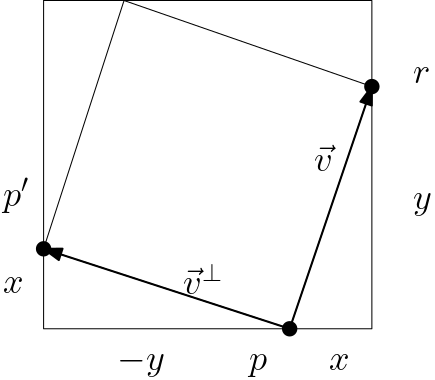
\includegraphics[width = 0.35\textwidth]{theory/v_square.png}
    \caption{Computing the coordinates of $\vec v^\perp$ given the guard $g$ and the reflex vertex $r(x, y)$.}
    \label{fig:vsquare}
\end{figure}

We know that the norm of the gradient is $||\bigtriangledown f|| = \frac{b^2}{2a}$. Since $\bigtriangledown f$ has the same direction as $\vec v^\perp$, we wish to normalise it from the norm of $\vec v^\perp$ with $\frac 1 a$. Therefore, the gradient for guard $g$ and one reflex vertex $r \in \mathit{Vis}(g)$ can be computed as $$\bigtriangledown f = \vec v^\perp \frac{b^2}{2a} \frac 1 a.$$

As mentioned before, the total gradient for guard $g$ and all the reflex vertices $r$ the guard can see is $$\bigtriangledown f = \sum_{r \in R(g)} \bigtriangledown \text{Area}_r, R(g) = \{\text{reflex vertices of } P \text{ seen by }g\}.$$

The new position $g'$ of guard $g$ based on all the reflex vertices it can see is: 
\begin{equation}
    g' = g + \alpha\bigtriangledown f.
    \label{eq:l}
\end{equation}

\newpage
\subsection{Guarding the Polygon with Multiple Guards}
In this subsection we will investigate how to generalise the computation of gradient descent to multiple guards.

\subsubsection{Computing the Gradient for Two Guards}
Let point $g_1$ be the guard we have previously computed the gradient for. Let point $g_2$ be another guard in the polygon. The position of $g_2$ is optimised around reflex vertex $r_2$, as seen in Figure \ref{fig:poly_gradient}. Guard $g_2$ sees a part of the visibility region already seen by $g_1$. Let the shared seen region be $\triangle_2$, and the region that is only visible by $g_1$ be $\triangle_1$.

\begin{figure}[h!]
    \centering
    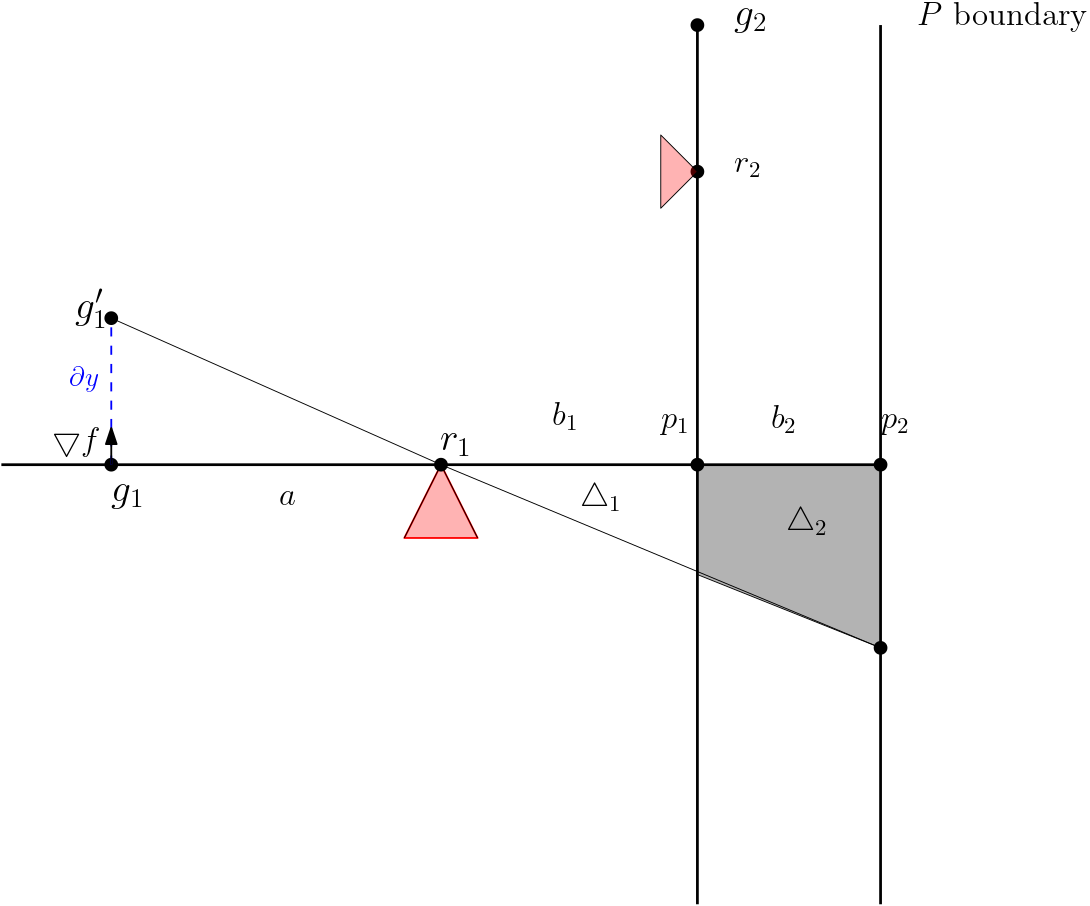
\includegraphics[width = 0.6\textwidth]{theory/gradient3.png}
    \caption{Canonical gradient construction for when the visible area of $g_1'$ is also seen by guard $g_2$.}
    \label{fig:poly_gradient}
\end{figure}

The visibility regions of guards $g_1$ and $g_2$ are computed. Let $p$ be the intersection point between them. Let $d$ be the point seen by $g_1$ on the polygon boundary. Point $p$ divides the segment seen by $g_1$ behind the reflex vertex $r_1$ into two subsegments $\overline{r_1p_1}$ and $\overline{p_1p_2}$. The lengths of the subsegments are $b_1$ and $b_2$, respectively, with $b_1 + b_2 = b$. Recall that $b$ is the distance between the reflex vertex $r_1$ and the polygon boundary. Thus,  $b_2$ corresponds to the length of the shared seen segment.

As before in equation \ref{eq:ardd}, the area seen by $g_1$ is $$\text{Area}_{\triangle_1 + \triangle_2} = (b_1 + b_2)^2\frac{\partial y}{2a}.$$
However, $\triangle_2$ is already seen by guard $g_2$. Since this area is already covered, we are only interested in how $g_1$ can cover the remaining $\triangle_1$. So, we do not need to take $\triangle_2$ into account when computing the gradient of $g_1$. We thus need to subtract the area of $\triangle_2$ from the total area seen by $g_1$. 

First, we need to compute the shared area seen $\triangle_2$ as:
\begin{align}
    \text{Area}_{\triangle_2} &= \text{Area}_{\triangle_1 + \triangle_2} - \text{Area}_{\triangle_2} \\
                              &= (b_1 + b_2)^2\frac{\partial y}{2a} - b_1^2\frac{\partial y}{2a} \\
                              &= \left[(b_1 + b_2)^2 - b_1^2\right]\frac{\partial y}{2a}. \label{eq:multiple_areas} 
\end{align}
Then, we can compute the area $\triangle_1$ seen exclusively by $g_1$ by subtracting the shared area of $\triangle_2$ from the total area seen by $g_1$: 
\begin{align*}
    \text{Area}_{\triangle_1} &= \text{Area}_{\triangle_1 + \triangle_2} - \text{Area}_{\triangle_1} \\
                              &= (b_1 + b_2)^2\frac{\partial y}{2a} - \left[(b_1 + b_2)^2 - b_1^2\right]\frac{\partial y}{2a} \\
    \text{Area}_{\triangle_1} &= b_1^2\frac{\partial y}{2a}. 
\end{align*}

\subsubsection{Computing the Gradient for Multiple Guards}
We can now generalise the gradient computation to $m$ guards and intersection points. Let $g$ be the guard whose position we wish to optimise around reflex vertex $r$ as before. Let the areas highlighted in blue in Figure \ref{fig:general_gradient} be the parts of the visibility region of $g$ that are also seen by the other $m - 1$ guards. Let the visibility region of $g$ intersect other guards' visibility regions in $m$ intersection points $p_1, p_2, ..., p_m$. Let the distance from the reflex vertex $r$ to the intersection points be $b_{11}, b_{12}, ..., b_{m1}, b$.

\begin{figure}[h!]
    \centering
    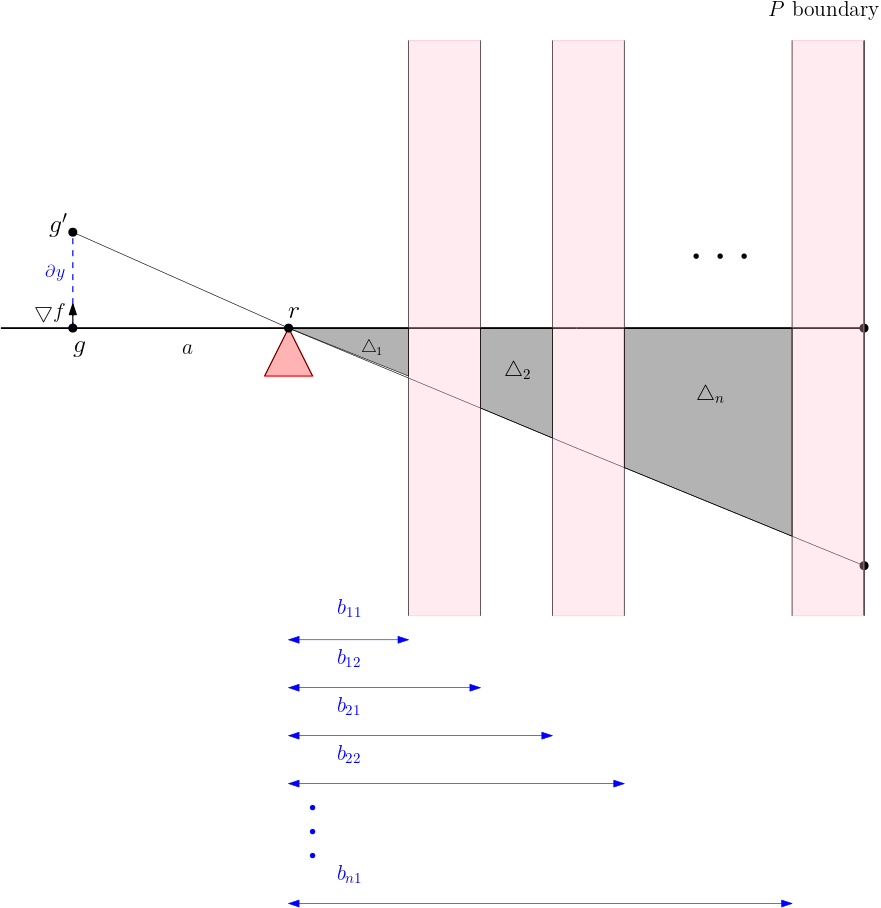
\includegraphics[width = 0.7\textwidth]{theory/gradient4.png}
    \caption{Canonical gradient construction for where the pink parts of the visible area of $g$ are also seen by other guards. The gray polygons $\triangle_1, \triangle_3, ..., \triangle_{m - 1}$ are the areas that are exclusively seen by $g$.}
    \label{fig:general_gradient} 
\end{figure}

We can now generalise equation \ref{eq:multiple_areas}. Namely, we need to subtract the areas that are seen by other guards from the total area seen by guard $g$. 

We start to move in the direction from the polygon boundary to reflex vertex $r$. We know the intersection points $p_{m - 1} ..., p_3, p_1$ of the shared seen regions with the visibility region of $g$. Thus, we can compute the distances $\overline{rp_{m - 1}}, ..., \overline{rp_3}, \overline{rp_1}$ between the reflex vertex $r$ and the beginning of the shared visibility regions. Analogously, we can compute the distances $\overline{rp_m}, ...,  \overline{rp_4}, \overline{rp_2}$ between the reflex vertex $r$ and the end of the shared visibility regions.

The areas of polygons $\triangle_1, \triangle_2, ..., \triangle_m$ do not grow linearly. For this reason, we cannot simply subtract the sum of the shared areas from the total area seen by $g$. An explanation about why this is the case is given in Figure \ref{fig:areas}. Take overlapping polygons $s_1, s_2, s_3, s_4$ with areas $\text{Area}_{s_1} = 2$, $\text{Area}_{s_2} = 3$, $\text{Area}_{s_3} = 4$, $\text{Area}_{s_4} = 5$. We want to compute the area of polygons $s_1$ and $s_2$. However, it is incorrect to simply add their areas together as $\text{Area}_{s_1 + s_3} = 2 + 4 = 6$, as $s_2$ is overlapping in between them. Instead, from the total area $\text{Area}_{s_1 + s_2 + s_3 + s_4} = \text{Area}_{s_4} = 5$ we can sequentially subtract the areas we are not interested in ($\text{Area}_{s_2}, \text{Area}_{s_4}$) and add the ones we are interested in ($\text{Area}_{s_1}, \text{Area}_{s_3}$). Namely, $\text{Area}_{s_1 + s_3} = \text{Area}_{s_1 + s_2 + s_3 + s_4} - \text{Area}_{s_4} + \text{Area}_{s_3} - \text{Area}_{s_2} + \text{Area}_{s_1} = 5 - 5 + 4 - 3 + 2 = 3$.

\begin{figure}[h!]
    \centering
    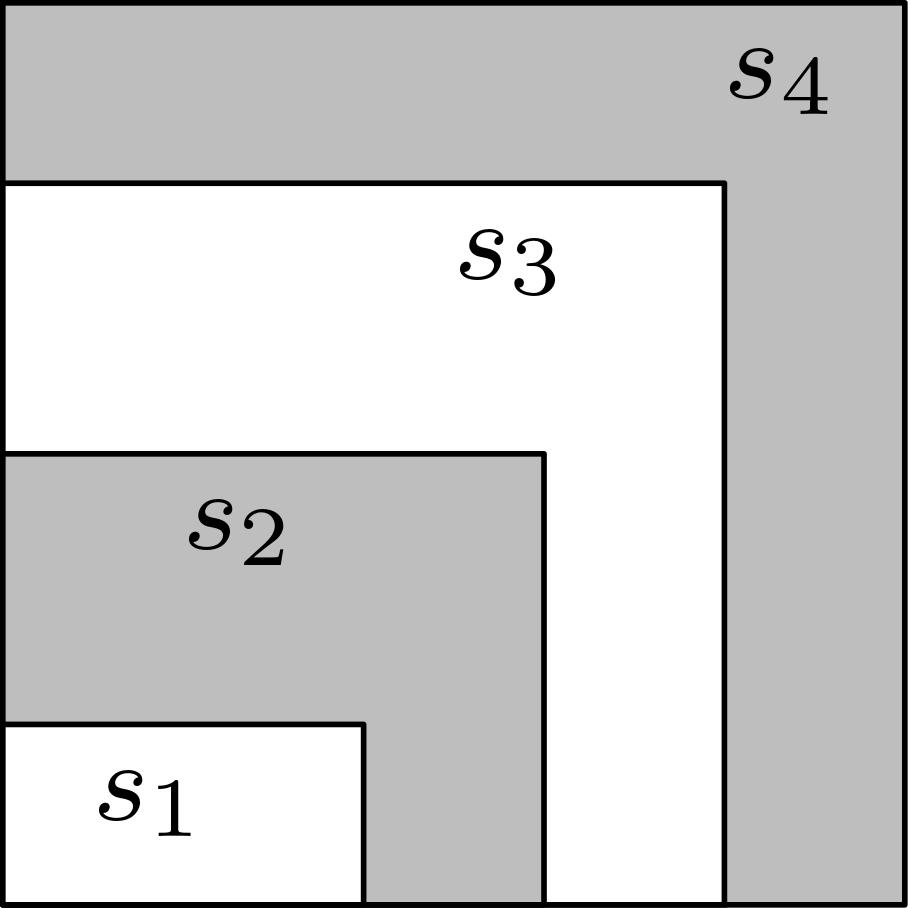
\includegraphics[width = 0.4\textwidth]{theory/area.png}
    \caption{Example for computing the area of overlapping polygons with areas $\text{Area}_{s_1} = 2$, $\text{Area}_{s_2} = 3$, $\text{Area}_{s_3} = 4$, $\text{Area}_{s_4} = 5$. It is incorrect to compute $\text{Area}_{s_1 + s_3} = 2 + 4 = 6$. Instead, $\text{Area}_{s_1 + s_3} = \text{Area}_{s_1 + s_2 + s_3 + s_4} - \text{Area}_{s_4} + \text{Area}_{s_3} - \text{Area}_{s_2} + \text{Area}_{s_1} = 5 - 5 + 4 - 3 + 2 = 3$.}
    \label{fig:areas}
\end{figure}

Similarly to Figure \ref{fig:areas}, we can compute the area seen exclusively by $g$. From the total area $\text{Area}_{\triangle_1 + \triangle_2, ..., \triangle_m}$ seen by $g$ we need to alternatively subtract the shared areas $\text{Area}_{\triangle_m}, ..., \text{Area}_{\triangle_4}, \text{Area}_{\triangle_2}$, then add the exclusively seen areas $\text{Area}_{\triangle_{m - 1}}, ..., \text{Area}_{\triangle_3}, \text{Area}_{\triangle_1}$.

% Figure \ref{fig:general_gradient} displays an example
% For each area seen by multiple guards, we know the length of the subsegments in between reflex vertex $r$ and the shared area beginning and ending, respectively. 
% In order to do so, we need to subtract the area $b_{i + 1}^2$ in between reflex vertex $r$ and the ending of the area, and then add back the area $b_i^2$ between $r$ and the beginning of the area. We need to repeat this process for each of the areas that are shared, in the direction starting from the polygon boundary to the reflex vertex.

This results in the fact that the area seen by $g$ exclusively can be computed as 
\begin{align*}
    \text{Area}_{\triangle_1 + \triangle_3 + ... + \triangle_{m - 1}} &= \text{Area}_{\triangle_1 + \triangle_2, ..., \triangle_m} - \text{Area}_{\triangle_{m - 1}} + \text{Area}_{\triangle_{m - 2}} - ... - \text{Area}_{\triangle_2} + \text{Area}_{\triangle_1} \\
                                                                      &= \left(b^2 - b_{m1}^2 + b_{(m - 1)2}^2 - ... - b_{12}^2 + b_{11}^2\right)\frac{\partial y}{2a}.
\end{align*}

Alternatively, if $\triangle_1$ is first seen by other guards (so $b_{11} = 0$), then all the signs are flipped. This claim can also be supported by the intuition of Figure \ref{fig:areas}. If we are interested in the areas of $s_2$ and $s_4$, then it is incorrect to compute them as $\text{Area}_{s_2 + s_4} = 3 + 5 = 8$. This is because $s_1$ and $s_3$ are overlapping in between them.  Instead, $\text{Area}_{s_2 + s_4} = \text{Area}_{s_1 + s_2 + s_3 + s_4} + \text{Area}_{s_4} - \text{Area}_{s_3} + \text{Area}_{s_2} - \text{Area}_{s_1} = 5 + 5 - 4 + 3 - 2 = 7$.

\subsection{Momentum}

In this section we introduce the concept of momentum. Its aim is to smoothen out the large noisy jumps in the gradient descent computation \cite{goodfelow2016deep}. Momentum builds upon the idea of considering the past states of the gradient descent computation. In this way, the past states create ``inertia'' to the newly computed gradient state. This results in the overall optimisation trajectory to be smoother.

So, the position $g_i$ at iteration $i$ of a guard $g$ will not be calculated anymore based only on the current computation of gradient descent. Instead, it will also take into account past values of gradient descent. In order to decide how much past states influence the value of the current position, we will take each gradient value with a weight.

Let $M_i$ be the momentum for a guard per iteration $i$. Let $\Delta f_i$ be the computation of the gradient descent in iteration $i$. Let the weight of a gradient descent value be a hyperparameter $\gamma$. 
As such, we can take into account the value of the previous gradient $\Delta_{i - 1}$ with weight $\gamma$. However, we still want the current gradient $\Delta f_i$ to influence the guard's movement. This can happen with a weight of $1 - \gamma$. So, the computation for the momentum at iteration $i$ becomes $$M_i = \gamma M_{i - 1} + (1 - \gamma)\Delta f_i.$$

Let $$M_0 = (1 - \gamma) \Delta f_0.$$. We can then check for correctness how  the next iterations of the momentum are carried out:
\begin{align*}
    M_1 &= \gamma M_0 + (1 - \gamma) \Delta f_1 \\
        &= \gamma (1 - \gamma) \Delta f_0 + (1 - \gamma) \Delta f_1 \\
        &= (1 - \gamma) (\gamma \Delta f_0 + \Delta f_1) \\
    M_2 &= \gamma M_1 + (1 - \gamma) \Delta f_2 \\
        &= \gamma (1 - \gamma) (\gamma \Delta f_0 + \Delta f_1) + (1 - \gamma) \Delta f_2 \\
        &= (1 - \gamma) (\gamma^2 \Delta f_0 + \gamma \Delta f_1 + \Delta f_2) \\
    ... \\
    M_i &= \gamma M_{i - 1} + (1 - \gamma) \Delta f_i \\
        &= (1 - \gamma) (\gamma^i \Delta f_0 + \gamma^{i - 1} \Delta f_1 + ... + \gamma \Delta f_{i - 1} + \Delta f_i) \\
\end{align*}

In this way, our momentum computation exponentially decreases the influence of a past state over the guard's current movement. So, the previous value of the momentum will exert its inertia with $\gamma$ influence over the new value of the momentum.

Similarly, the new position $g_i$ of guard $g$ will now be calculated as $$g_i = g_{i - 1} + \alpha M_i.$$